% !TeX root = enterprise-architecture-digital-blueprint.tex
% !TeX encoding = UTF-8
\chapter{Arsitektur Bisnis Saat Ini: Capability Map dan Value Stream}

\section*{Tujuan Pembelajaran}
\begin{itemize}
  \item Membedakan kapabilitas bisnis, proses bisnis, dan unit organisasi.
  \item Menyusun \textit{capability map} dua tingkat dan satu \textit{value stream} utama untuk organisasi \textit{capstone}.
  \item Menilai kondisi kapabilitas dalam \textit{heatmap} yang didukung bukti.
\end{itemize}

\section{Pendahuluan}

Misalkan direksi Medikara membuka rapat anggaran 2027 dengan satu pertanyaan:
kemampuan apa yang paling menghambat strategi ``Satu Pasien, Satu Rekam Medis''?
Para kepala unit datang membawa bagan organisasi, kumpulan \textit{Standard
Operating Procedure} (SOP), dan daftar permintaan aplikasi. Bagan menjawab siapa
melapor kepada siapa. SOP menjawab langkah kerja di satu tempat. Daftar permintaan
menjawab apa yang ingin dibeli tiap unit. Tidak satu pun menjawab pertanyaan direksi.

Akibatnya terasa setiap hari. Lima rumah sakit hasil akuisisi punya Sistem Informasi
Manajemen Rumah Sakit (SIMRS) dengan versi berbeda dan cara pendaftaran yang berbeda.
Dua unit dapat membeli aplikasi untuk kemampuan yang sama, sementara
kemampuan menjaga identitas pasien lintas fasilitas tidak punya satu pemilik pun.
Panduan \textit{Business Architecture Body of Knowledge} (BIZBOK) memberi contoh
serupa: sebuah perusahaan membangun beberapa solusi pendaftaran yang saling bersaing
untuk pelanggan yang sama, dan hasilnya kerumitan serta ketidakpuasan pelanggan
\cite{bizbok15}. Masalah semacam ini baru terlihat bila organisasi dibaca lewat
kemampuan dan nilai yang dihasilkannya.
\IfFileExists{../figures/ch05-diagram-konsep.png}{%
Kapabilitas dipetakan ke tahap value stream yang didukungnya.
Urutan tahap nilai tidak mengubah kapabilitas menjadi urutan proses.
Gambar \ref{fig:ch05-ilustrasi-bab} merangkum hubungan komponen dan konsep utama bab ini.
\begin{figure}[!htb]
  \centering
  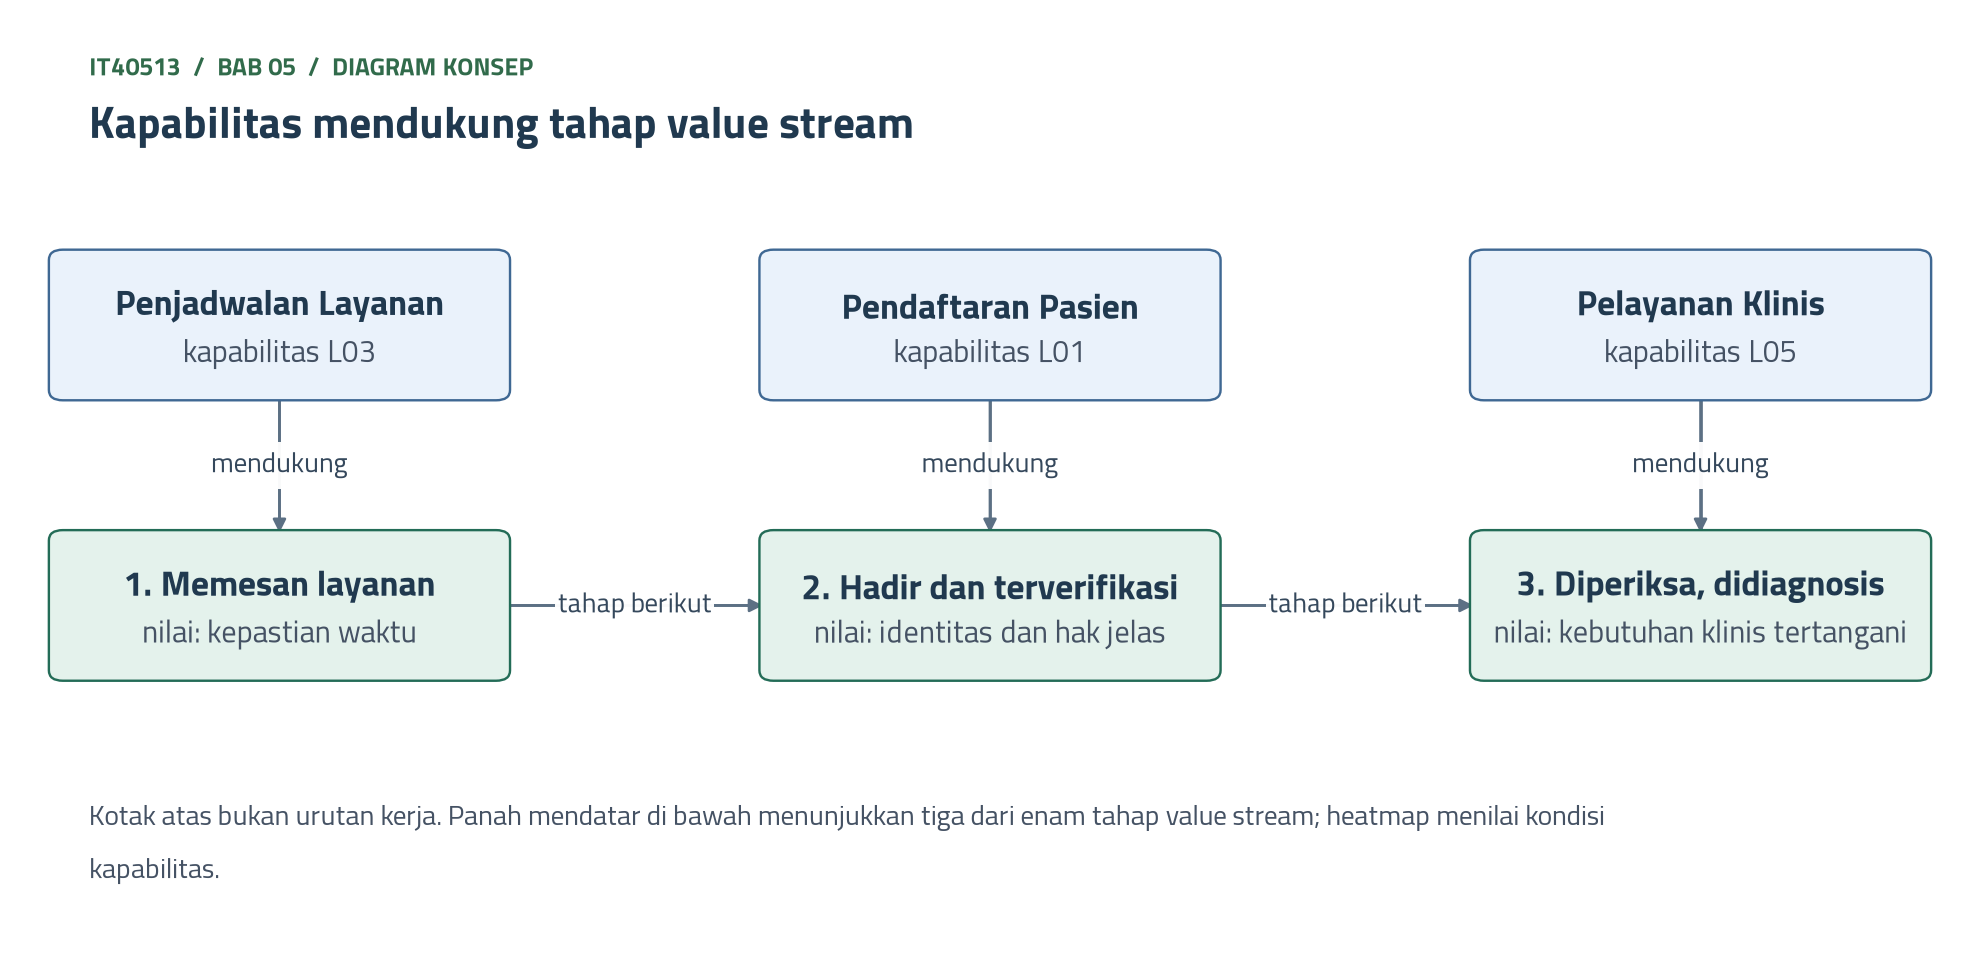
\includegraphics[width=\textwidth]{../figures/ch05-diagram-konsep.png}
  \caption{Kapabilitas mendukung tahap value stream}
  \label{fig:ch05-ilustrasi-bab}
\end{figure}
}{}

Bab ini memotret arsitektur bisnis saat ini, yaitu pekerjaan fase B dalam
\textit{Architecture Development Method} (ADM) milik The Open Group Architecture
Framework (TOGAF) \cite{togaf10}. Rujukan utamanya BIZBOK versi 15 \cite{bizbok15}.
Panduan itu memandang arsitektur bisnis sebagai gambaran utuh tentang kapabilitas,
penyampaian nilai ujung ke ujung, informasi, dan struktur organisasi, beserta
hubungannya dengan strategi, produk, kebijakan, inisiatif, dan \textit{stakeholder}.
Khosroshahi dan rekan meneliti praktik dan kasus pakai \textit{capability map} dalam
pengelolaan arsitektur \textit{enterprise}; artikel itu dianjurkan sebagai bacaan
pendamping \cite{c05-khosroshahi2018}. Pembahasan berjalan dari kapabilitas,
\textit{capability map}, \textit{value stream}, pemetaan silang, sampai
\textit{heatmap}. Peta Medikara pada bab ini adalah model latihan yang disusun untuk
kelas, bukan salinan model referensi industri BIZBOK.

\section{Kapabilitas Bisnis}

Kapabilitas bisnis adalah kemampuan yang dimiliki organisasi untuk mencapai suatu
hasil. Namanya menyatakan apa yang mampu dilakukan, bukan bagaimana melakukannya,
siapa pelaksananya, di mana tempatnya, atau aplikasi apa yang dipakai. Kapabilitas
diwujudkan oleh empat unsur: orang dan unit, proses, informasi, serta sumber daya
seperti aplikasi dan peralatan. Unsur-unsur itu dapat berganti, sedangkan kemampuannya
tetap diperlukan. BIZBOK memberi contoh perusahaan asuransi berusia 100 tahun:
kemampuan seperti \textit{Customer Management}, \textit{Insurance Policy Management},
dan \textit{Claims Management} sudah ada sebelum ada otomasi, dan masih ada sampai
sekarang \cite{bizbok15}.

Peta yang hanya mencantumkan aplikasi kehilangan unsur penting seperti keterampilan
petugas, wewenang koreksi data, dan prosedur rujukan. Pembelian aplikasi memperbaiki
sebagian unsur, tetapi belum tentu meningkatkan kemampuan layanan secara keseluruhan.

Analoginya seperti kemampuan memasak dalam keluarga. Memasak adalah kemampuan.
Mengikuti resep adalah proses. Anggota keluarga yang memasak adalah pelaksana. Kompor
dan bahan adalah sumber daya. Mengganti kompor tidak otomatis mengajarkan keterampilan
atau memperbaiki pembagian tugas di dapur.

Gambar \ref{fig:ch05-kapabilitas} memperlihatkan keempat unsur itu pada satu
kapabilitas Medikara.

\begin{figure}[!htb]
  \centering
  \begin{tikzpicture}[
  font=\scriptsize,
  induk/.style={draw, rounded corners, fill=praditagreen!15, align=center,
                text width=4.2cm, minimum height=1.1cm, font=\scriptsize\bfseries},
  kotak/.style={draw, rounded corners, fill=blue!8, align=center, text width=2.4cm,
                minimum height=1.35cm, font=\scriptsize\bfseries},
  panah/.style={-{Stealth[length=2mm]}, thick}
]
  \node[induk] (kap) at (5.8,0)
    {Penjadwalan Layanan (CAP-L03)\\{\tiny\mdseries kapabilitas: apa yang dilakukan}};
  \node[font=\tiny, gray, anchor=west, align=left] at (8.15,0)
    {relatif stabil\\selama bertahun-tahun};

  \node[kotak] (orang) at (1.45,-2.6)
    {Orang dan unit\\{\tiny\mdseries petugas loket lima rumah sakit,
     petugas telepon, tim Medikara+}};
  \node[kotak] (proses) at (4.35,-2.6)
    {Proses\\{\tiny\mdseries lima SOP janji temu yang berbeda}};
  \node[kotak] (info) at (7.25,-2.6)
    {Informasi\\{\tiny\mdseries identitas pasien dan jadwal praktik dokter}};
  \node[kotak] (sumber) at (10.15,-2.6)
    {Sumber daya\\{\tiny\mdseries lima versi SIMRS, aplikasi Medikara+, telepon}};

  \draw[panah] (orang.north) -- ($(kap.south)+(-1.5,0)$);
  \draw[panah] (proses.north) -- ($(kap.south)+(-0.5,0)$);
  \draw[panah] (info.north) -- ($(kap.south)+(0.5,0)$);
  \draw[panah] (sumber.north) -- ($(kap.south)+(1.5,0)$);
  \node[font=\tiny, fill=white, inner sep=1pt] at (5.8,-1.15) {diwujudkan oleh};

  \begin{scope}[on background layer]
    \node[draw=gray, dashed, rounded corners, fit=(orang)(sumber), inner sep=5pt] (bawah) {};
  \end{scope}
  \node[font=\tiny, gray, anchor=north] at (bawah.south)
    {bagaimana, oleh siapa, dan dengan apa: berubah saat reorganisasi, revisi SOP,
     atau penggantian aplikasi};
\end{tikzpicture}

  \caption{Kapabilitas Penjadwalan Layanan dan empat unsur yang mewujudkannya}
  \label{fig:ch05-kapabilitas}
\end{figure}

Dua contoh dari Medikara Health:

\begin{enumerate}
  \item Misalkan 28 persen dari sekitar 1,2 juta kunjungan per tahun, atau 336.000 janji temu,
        dipesan lewat Medikara+, sedangkan 72 persen sisanya lewat telepon dan loket di lima
        rumah sakit dan 18 klinik pratama.
        Ketiga saluran itu mewujudkan satu kapabilitas, yaitu Penjadwalan Layanan. Bila
        peta memakai nama saluran atau aplikasi, satu kemampuan tampak sebagai tiga hal,
        dan anggaran perbaikannya terpecah ke tiga pemilik.
  \item Misalkan pada 2027 Medikara memusatkan layanan telepon janji temu kelima rumah
        sakit ke satu unit berisi 40 petugas. Bagan organisasi berubah: lima seksi hilang
        dan satu unit baru muncul. Kapabilitas Penjadwalan Layanan tetap berkode CAP-L03,
        sehingga pemetaan pada Bab 6 dan Bab 7 tidak perlu ditulis ulang. Hanya kolom
        pelaksana yang berubah, dari lima baris menjadi satu.
\end{enumerate}

Tiga hal sering tertukar: kapabilitas, proses, dan unit organisasi. Dua hal lain ikut
tercampur: sumber daya dan keluaran. Pembagiannya begini. Tabel
\ref{tab:ch05-lima-jenis} memisahkan kelimanya lewat pertanyaan yang dijawab dan pemicu
perubahannya.

\begin{table}[!htb]
  \centering
  \caption{Lima hal yang sering tercampur saat memetakan bisnis}
  \label{tab:ch05-lima-jenis}
  \small
  \begin{tabularx}{\textwidth}{>{\raggedright\arraybackslash}p{2.0cm}>{\raggedright\arraybackslash}X>{\raggedright\arraybackslash}p{2.8cm}>{\raggedright\arraybackslash}p{2.9cm}}
    \hline
    \textbf{Jenis} & \textbf{Contoh Medikara} & \textbf{Pertanyaan} & \textbf{Berubah ketika} \\
    \hline
    Kapabilitas & Penjadwalan Layanan & Apa yang mampu dilakukan? & Strategi atau model bisnis berubah \\
    \hline
    Proses bisnis & Memeriksa slot, memilih dokter, lalu mengonfirmasi jadwal & Bagaimana pekerjaan berlangsung? & SOP direvisi \\
    \hline
    Unit organisasi & Seksi pendaftaran rumah sakit Bekasi & Siapa yang menjalankan? & Reorganisasi \\
    \hline
    Sumber daya & Medikara+, telepon, lima SIMRS & Dengan apa dijalankan? & Aplikasi atau alat diganti \\
    \hline
    Keluaran & Pesan konfirmasi jadwal & Apa hasil satu kali kerja? & Setiap kali proses berjalan \\
    \hline
  \end{tabularx}
\end{table}

Perbedaan kapabilitas dan keluaran paling sering terlewat. ``Laporan bulanan direksi''
adalah keluaran, sedangkan
Pelaporan Manajemen adalah kemampuan menghasilkan dan menjaga laporan yang dapat dipercaya.
Laporan yang baru terbit pada hari kerja ke-12 (Bab 6) menjadi bukti kondisi kapabilitas,
bukan definisinya.

Memisahkan kapabilitas dari pelaksana dan aplikasi punya dua konsekuensi. Pertama, peta
bertahan lebih lama. Misalkan lima SIMRS kelak dilebur menjadi satu. Lima baris hilang dari
katalog aplikasi Bab 7, tetapi 15 kapabilitas pada peta Medikara tetap sama. Kedua, peta
tidak menjawab sendiri pertanyaan ``aplikasi mana yang dipakai''. Tim harus memelihara
pemetaan tambahan. Misalkan katalog awal memuat 8 aplikasi. Dengan 15 kapabilitas, ada
$15 \times 8 = 120$ sel yang harus ditinjau. Itulah harga dari peta yang stabil.

\subsection*{Aturan penamaan}

Aturan penamaan perlu disepakati sejak awal. Nama berupa frasa benda yang menjelaskan
kemampuan, misalnya Klaim dan Penjaminan atau Pelayanan Klinis. Tingkatnya tidak boleh
dicampur: ``Pelayanan Pasien'' tidak sebanding dengan ``Mengeklik tombol simpan''. Setiap
nama memiliki definisi satu kalimat agar tim berbeda memakai arti yang sama. Setiap
kapabilitas juga diberi kode tetap, misalnya CAP-L01, seperti pada
\berkas{sources/chapter04/konvensi-penamaan-model.md}. Dengan kode tetap, nama dapat
diperbaiki tanpa memutus pemetaan pada Bab 6 dan Bab 7. Tabel \ref{tab:ch05-aturan-nama}
memberi contoh perbaikan nama.

\begin{table}[!htb]
  \centering
  \caption{Memperbaiki nama yang belum menyatakan kapabilitas}
  \label{tab:ch05-aturan-nama}
  \small
  \begin{tabularx}{\textwidth}{>{\raggedright\arraybackslash}p{3.8cm}>{\raggedright\arraybackslash}X>{\raggedright\arraybackslash}p{3.8cm}}
    \hline
    \textbf{Nama awal} & \textbf{Masalah} & \textbf{Nama kapabilitas} \\
    \hline
    Janji temu lewat telepon & Menyebut saluran & Penjadwalan Layanan \\
    \hline
    Modul Resep SIMRS & Menyebut aplikasi & Layanan Farmasi dan Laboratorium \\
    \hline
    Bagian Klaim & Menyebut unit & Klaim dan Penjaminan \\
    \hline
    Mengisi formulir verifikasi & Langkah proses, tingkatnya terlalu rendah & Bagian dari Pendaftaran Pasien \\
    \hline
    Laporan bulanan direksi & Menyebut keluaran & Pelaporan Manajemen \\
    \hline
  \end{tabularx}
\end{table}

\section{Menyusun Capability Map}

\textit{Capability map} adalah gambar satu halaman yang mengelompokkan seluruh kemampuan
organisasi ke dalam beberapa tingkat. Tingkat 1 memberi kelompok besar. Tingkat 2 membagi
tiap kelompok menjadi kemampuan yang lebih spesifik. Hubungan induk dan anak menyatakan
penguraian, bukan urutan waktu. Karena itu peta tidak memakai panah proses, sebab satu
kapabilitas dapat mendukung banyak proses sekaligus. BIZBOK membahas penyusunan peta ini
beserta pemetaan silangnya ke domain lain pada bagian 2.2 \cite{bizbok15}. Dua tingkat
sudah memadai untuk \textit{capstone}. Tingkat yang lebih rinci hanya dibuat ketika sebuah
keputusan membutuhkannya.

Analoginya seperti daftar isi perpustakaan. Kelompok besar membantu menemukan topik,
sedangkan subkelompok memberi rincian. Daftar isi tidak menunjukkan urutan pengunjung
membaca semua buku. Bila setiap rak memakai nama yang tumpang tindih, pembaca sulit
mengetahui lokasi informasi yang benar.

Gambar \ref{fig:ch05-peta-kapabilitas} memperlihatkan peta dua tingkat Medikara saat ini.

\begin{figure}[!htb]
  \centering
  \begin{tikzpicture}[
  font=\scriptsize,
  kap/.style={draw, fill=blue!8, text width=3.3cm, minimum height=0.5cm,
              align=center, font=\tiny, inner sep=2pt},
  tambal/.style={kap, fill=gray!35, dashed},
  judul/.style={font=\scriptsize\bfseries, align=center, text width=3.5cm}
]
  \draw[rounded corners, fill=praditagreen!15] (0,0.75) rectangle (3.8,-4.45);
  \draw[rounded corners, fill=praditagreen!15] (4.0,0.75) rectangle (7.8,-4.45);
  \draw[rounded corners, fill=praditagreen!15] (8.0,0.75) rectangle (11.8,-4.45);
  \node[judul] at (1.9,0.35) {CAP-S\\Kapabilitas Strategis};
  \node[judul] at (5.9,0.35) {CAP-L\\Kapabilitas Layanan Pasien};
  \node[judul] at (9.9,0.35) {CAP-P\\Kapabilitas Pendukung};

  \node[kap] at (1.9,-0.35) {S01 Manajemen Strategi};
  \node[kap] at (1.9,-0.97) {S02 Pengelolaan Kepatuhan};

  \node[kap] at (5.9,-0.35) {L01 Pendaftaran Pasien};
  \node[tambal] at (5.9,-0.97) {L02 Penerbitan Nomor Rekam Medis Lokal};
  \node[kap] at (5.9,-1.59) {L03 Penjadwalan Layanan};
  \node[kap] at (5.9,-2.21) {L04 Pengelolaan Rekam Medis};
  \node[kap] at (5.9,-2.83) {L05 Pelayanan Klinis};
  \node[kap] at (5.9,-3.45) {L06 Layanan Farmasi dan Laboratorium};
  \node[kap] at (5.9,-4.07) {L07 Telekonsultasi};

  \node[kap] at (9.9,-0.35) {P01 Klaim dan Penjaminan};
  \node[kap] at (9.9,-0.97) {P02 Pengelolaan Akses Pengguna};
  \node[kap] at (9.9,-1.59) {P03 Pelaporan Manajemen};
  \node[kap] at (9.9,-2.21) {P04 Keuangan dan Akuntansi};
  \node[kap] at (9.9,-2.83) {P05 Pengelolaan Tenaga Kerja};
  \node[tambal] at (9.9,-3.45) {P06 Rekonsiliasi Data Manual Antarfasilitas};

  \draw[fill=praditagreen!15] (0.6,-4.82) rectangle (0.9,-5.02);
  \node[font=\tiny, anchor=west] at (0.95,-4.92) {tingkat 1 (kelompok)};
  \draw[fill=blue!8] (4.0,-4.82) rectangle (4.3,-5.02);
  \node[font=\tiny, anchor=west] at (4.35,-4.92) {tingkat 2};
  \draw[fill=gray!35, dashed] (6.6,-4.82) rectangle (6.9,-5.02);
  \node[font=\tiny, anchor=west] at (6.95,-4.92)
    {kapabilitas tambalan: ada karena data terpecah};
\end{tikzpicture}

  \caption{\textit{Capability map} Medikara saat ini: tiga kelompok tingkat 1 dan 15
           kapabilitas tingkat 2 berkode tetap}
  \label{fig:ch05-peta-kapabilitas}
\end{figure}

Dua contoh dari Medikara Health:

\begin{enumerate}
  \item Misalkan wawancara dan SOP dari lima rumah sakit menghasilkan 41 usulan nama. Dari
        jumlah itu, 14 ternyata nama aplikasi atau unit, 9 adalah langkah proses, dan 3
        adalah sinonim, misalnya Registrasi, Admisi, dan Pendaftaran Rawat Jalan. Sesudah
        dibersihkan, tersisa $41 - 14 - 9 - 3 = 15$ kapabilitas tingkat 2.
  \item Misalkan pemeriksaan hak penjaminan dikerjakan di loket 5 rumah sakit dan 18 klinik
        pratama, sedangkan penyelesaian klaim dikerjakan bagian klaim pusat. Peta tetap
        mencatat satu kapabilitas, yaitu Klaim dan Penjaminan, dengan dua kelompok pelaksana.
        Tanpa pemeriksaan batas ini, pekerjaan di 23 fasilitas itu tercatat ganda.
\end{enumerate}

Tabel \ref{tab:ch05-kelompok} memperlihatkan pertanyaan pemandu tiap kelompok.

\begin{table}[!htb]
  \centering
  \caption{Tiga kelompok tingkat 1 pada peta Medikara}
  \label{tab:ch05-kelompok}
  \small
  \begin{tabularx}{\textwidth}{>{\raggedright\arraybackslash}p{2.3cm}>{\raggedright\arraybackslash}X>{\raggedright\arraybackslash}X>{\raggedright\arraybackslash}p{1.2cm}}
    \hline
    \textbf{Tingkat 1} & \textbf{Pertanyaan pemandu} & \textbf{Contoh tingkat 2} & \textbf{Jumlah} \\
    \hline
    Strategis & Ke mana organisasi menuju, dan aturan apa yang mengikatnya? & Manajemen Strategi, Pengelolaan Kepatuhan & 2 \\
    \hline
    Layanan Pasien & Kemampuan apa yang langsung dirasakan pasien? & Pendaftaran Pasien, Pelayanan Klinis & 7 \\
    \hline
    Pendukung & Kemampuan apa yang menopang semua layanan? & Klaim dan Penjaminan, Pelaporan Manajemen & 6 \\
    \hline
  \end{tabularx}
\end{table}

Pengelompokan itu membantu pembacaan, tetapi tidak menjadi penilaian otomatis atas
prioritas. Pengelolaan Akses Pengguna berada di kelompok pendukung, tetapi dapat lebih
mendesak daripada perubahan pada layanan inti ketika ditemukan celah akses yang berat.

\subsection*{Model referensi sebagai titik awal}

Pertanyaan kemudian muncul: apakah peta harus disusun dari kertas kosong? Tidak harus.
Bagian 8 BIZBOK memuat model referensi industri yang berfungsi sebagai dasar untuk membangun
arsitektur bisnis sendiri. Bagian 8.3 memuat model industri kesehatan, dengan fokus pada
penyedia layanan diagnosis, pengobatan, dan pencegahan. Bagian 8.5 memuat model industri
asuransi, bagian 8.6 memuat model umum lintas industri, dan bagian 8.8 memuat model
pemerintahan \cite{bizbok15}. Model itu disediakan bagi anggota Business Architecture Guild
untuk pemakaian di organisasinya, sehingga isinya tidak disalin ke modul ini. Tim yang punya
akses memakainya sebagai daftar periksa. Tim lain memakai peta Medikara sebagai pembanding.

Memakai model referensi punya dua konsekuensi. Pertama, peta lebih cepat lengkap, karena
tim tidak lupa pada kemampuan yang jarang disebut dalam wawancara, misalnya Pengelolaan
Kepatuhan. Kedua, tim berisiko menyalin kemampuan yang tidak dikerjakan organisasinya.
Karena itu setiap baris dari model referensi ditanyakan kembali: apakah organisasi ini
benar-benar melakukannya, dan siapa pemiliknya?

\subsection*{Menguji peta}

Peta awal diuji dengan tiga pertanyaan. Apakah setiap kemampuan penting punya tempat? Apakah
dua nama menjelaskan kemampuan yang sama? Apakah penguraian anak cukup lengkap untuk
menjelaskan induknya? Tim memperbaiki definisi sebelum menambahkan rincian baru.

Bahan pengujian berasal dari wawancara, daftar layanan, kebijakan, SOP, dan laporan
kinerja. Analis bisnis memimpin penamaan. Analis teknologi membantu menemukan kemampuan yang
tersembunyi di dalam aplikasi atau \textit{spreadsheet}. Pemodel menjaga kode tetap, sehingga
perbaikan nama tidak memutus pemetaan pada bab berikutnya.

\begin{kasus}[title={Kasus Medikara Health: Kapabilitas Tambalan dan Kapabilitas yang Belum Ada}]
  Peta pada Gambar \ref{fig:ch05-peta-kapabilitas} memuat dua kotak bergaris putus-putus.
  Penerbitan Nomor Rekam Medis Lokal (CAP-L02) dan Rekonsiliasi Data Manual Antarfasilitas
  (CAP-P06) disebut di sini sebagai kapabilitas tambalan. Keduanya ada karena lima SIMRS
  tidak berbagi data. Namanya sengaja memuat kata ``lokal'' dan ``manual'', walaupun aturan
  penamaan biasanya melarang keterangan cara. Keterangan itu justru inti temuannya: pekerjaan
  tersebut menyita tenaga tetap, punya pelaksana, dan akan hilang bila akarnya diselesaikan.
  Keputusan menulisnya apa adanya adalah pilihan modul ini, bukan aturan BIZBOK.

  Peta juga dibaca dari sisi sebaliknya: apa yang dituntut strategi, tetapi tidak ada di
  peta? Tim mencatat tiga kemampuan:

  \begin{itemize}
    \item \textbf{Pengelolaan identitas pasien lintas fasilitas.} Pemilik bisnis konsep
          Pasien saat ini lima orang, sehingga tidak ada yang berwenang menetapkan satu
          aturan untuk seluruh jaringan (Bab 6).
    \item \textbf{Pengelolaan kemitraan ekosistem.} Hubungan dengan klinik mitra, asuransi,
          dan apotek daring ditangani per kontrak oleh tiap rumah sakit.
    \item \textbf{Wawasan pasien dan analitik.} Data pemakaian Medikara+ dan keluhan pasien
          belum dianalisis bersama.
  \end{itemize}

  Kemampuan yang tidak ada tidak dapat diberi warna pada \textit{heatmap}. Ketiganya dicatat
  sebagai daftar celah pada dokumen C2, lalu dibahas sebagai kandidat kapabilitas baru pada
  Bab 8.
\end{kasus}

\section{Value Stream}

\textit{Value stream} adalah rangkaian tahap ujung ke ujung yang menghasilkan nilai bagi satu
\textit{stakeholder} tertentu, dilihat dari sudut pandang penerima itu. Tim lebih dahulu
menetapkan penerima nilai, pemicu, dan nilai akhir, baru kemudian tahap-tahap di antaranya.
Setiap tahap memberi kemajuan yang dirasakan penerima, sehingga satu tahap dapat melibatkan
beberapa unit dan banyak proses. BIZBOK mencontohkan \textit{value stream} seperti
\textit{Settle Claim} dan \textit{Acquire Product}, dengan tahap seperti \textit{Validate
Eligibility} dan \textit{Finalize Agreement} \cite{bizbok15}. Bentuk namanya kata kerja dan
objek.

Penerima nilai menentukan isi tahap. Untuk rawat jalan, nilai pasien bukan ``formulir
dipindahkan'', melainkan akses layanan yang pasti, kebutuhan yang ditangani, dan tindak lanjut
yang jelas. Untuk klaim asuransi, penerimanya harus dinyatakan. ``Klaim dibayar'' bagi rumah
sakit berbeda dari ``kewajiban klaim diselesaikan secara sah'' bagi perusahaan asuransi.
Sudut pandang yang berubah mengubah batas tahap.

Analoginya seperti mengirim paket. Pengirim menilai tiga hal: paket dijemput, paket dalam
perjalanan, dan paket diterima. Perusahaan kurir punya banyak proses di dalamnya, seperti
penyortiran, pemuatan, dan pengaturan rute. Proses itu penting, tetapi pengirim tidak
menilainya satu per satu. Pengirim hanya tahu paketnya belum tiba.

Gambar \ref{fig:ch05-value-stream} memperlihatkan \textit{value stream} utama Medikara,
``Pasien menerima layanan rawat jalan'', beserta ukuran saat ini dan kapabilitas utamanya.
Tabel \ref{tab:ch05-tahap-nilai} merinci nilai dan kriteria selesai tiap tahap. Misalkan
angka ukuran berasal dari pengukuran awal di kelima rumah sakit pada 2026, dan angka keluhan
berasal dari catatan unit layanan pelanggan sepanjang 2025. Klaim pada tahap 5 adalah berkas
yang dikirim ke Badan Penyelenggara Jaminan Sosial (BPJS) Kesehatan.

\begin{figure}[!htb]
  \centering
  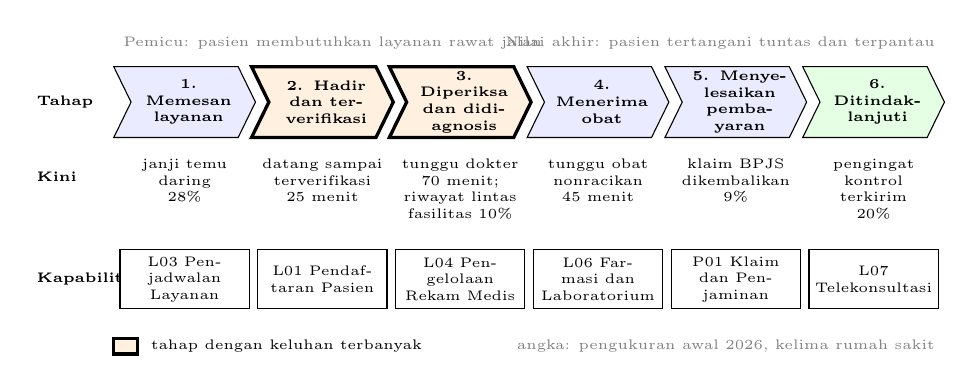
\begin{tikzpicture}[
  font=\scriptsize,
  tahap/.style={fill=blue!8, draw},
  tekan/.style={fill=orange!12, draw, very thick},
  isi/.style={text width=1.25cm, align=center, font=\tiny\bfseries},
  ukur/.style={text width=1.6cm, align=center, font=\tiny, anchor=north},
  kap/.style={draw, fill=white, text width=1.5cm, minimum height=0.75cm,
              align=center, font=\tiny, inner sep=2pt},
  label/.style={font=\tiny\bfseries, anchor=west}
]
  \node[font=\tiny, gray, anchor=west] at (1.1,1.2)
    {Pemicu: pasien membutuhkan layanan rawat jalan};
  \node[font=\tiny, gray, anchor=east] at (11.65,1.2)
    {Nilai akhir: pasien tertangani tuntas dan terpantau};

  \node[label] at (0,0.45) {Tahap};
  \node[label] at (0,-0.5) {Kini};
  \node[label] at (0,-1.8) {Kapabilitas};

  \draw[tahap] (1.10,0) -- ++(1.58,0) -- ++(0.22,0.45) -- ++(-0.22,0.45)
    -- ++(-1.58,0) -- ++(0.22,-0.45) -- cycle;
  \draw[tekan] (2.85,0) -- ++(1.58,0) -- ++(0.22,0.45) -- ++(-0.22,0.45)
    -- ++(-1.58,0) -- ++(0.22,-0.45) -- cycle;
  \draw[tekan] (4.60,0) -- ++(1.58,0) -- ++(0.22,0.45) -- ++(-0.22,0.45)
    -- ++(-1.58,0) -- ++(0.22,-0.45) -- cycle;
  \draw[tahap] (6.35,0) -- ++(1.58,0) -- ++(0.22,0.45) -- ++(-0.22,0.45)
    -- ++(-1.58,0) -- ++(0.22,-0.45) -- cycle;
  \draw[tahap] (8.10,0) -- ++(1.58,0) -- ++(0.22,0.45) -- ++(-0.22,0.45)
    -- ++(-1.58,0) -- ++(0.22,-0.45) -- cycle;
  \draw[tahap, fill=green!10] (9.85,0) -- ++(1.58,0) -- ++(0.22,0.45)
    -- ++(-0.22,0.45) -- ++(-1.58,0) -- ++(0.22,-0.45) -- cycle;

  \node[isi] at (2.05,0.45) {1. Memesan layanan};
  \node[isi] at (3.80,0.45) {2. Hadir dan terverifikasi};
  \node[isi] at (5.55,0.45) {3. Diperiksa dan didiagnosis};
  \node[isi] at (7.30,0.45) {4. Menerima obat};
  \node[isi] at (9.05,0.45) {5. Menyelesaikan pembayaran};
  \node[isi] at (10.80,0.45) {6. Ditindak\-lanjuti};

  \node[ukur] at (2.00,-0.15) {janji temu daring\\28\%};
  \node[ukur] at (3.75,-0.15) {datang sampai terverifikasi\\25 menit};
  \node[ukur] at (5.50,-0.15) {tunggu dokter 70 menit; riwayat lintas fasilitas 10\%};
  \node[ukur] at (7.25,-0.15) {tunggu obat nonracikan\\45 menit};
  \node[ukur] at (9.00,-0.15) {klaim BPJS dikembalikan\\9\%};
  \node[ukur] at (10.75,-0.15) {pengingat kontrol terkirim\\20\%};

  \node[kap] at (2.00,-1.8) {L03 Penjadwalan Layanan};
  \node[kap] at (3.75,-1.8) {L01 Pendaftaran Pasien};
  \node[kap] at (5.50,-1.8) {L04 Pengelolaan Rekam Medis};
  \node[kap] at (7.25,-1.8) {L06 Farmasi dan Laboratorium};
  \node[kap] at (9.00,-1.8) {P01 Klaim dan Penjaminan};
  \node[kap] at (10.75,-1.8) {L07 Telekonsul\-tasi};

  \draw[fill=orange!12, very thick] (1.1,-2.55) rectangle (1.4,-2.75);
  \node[font=\tiny, anchor=west] at (1.45,-2.65) {tahap dengan keluhan terbanyak};
  \node[font=\tiny, gray, anchor=east] at (11.65,-2.65)
    {angka: pengukuran awal 2026, kelima rumah sakit};
\end{tikzpicture}

  \caption{\textit{Value stream} ``Pasien menerima layanan rawat jalan'' saat ini, dengan
           ukuran dan satu kapabilitas utama untuk tiap tahap}
  \label{fig:ch05-value-stream}
\end{figure}

\begin{table}[!htb]
  \centering
  \caption{Nilai, kriteria selesai, ukuran, dan keluhan tiap tahap rawat jalan}
  \label{tab:ch05-tahap-nilai}
  \small
  \begin{tabularx}{\textwidth}{>{\raggedright\arraybackslash}p{2.5cm}>{\raggedright\arraybackslash}X>{\raggedright\arraybackslash}p{2.6cm}>{\raggedright\arraybackslash}p{2.7cm}r}
    \hline
    \textbf{Tahap} & \textbf{Nilai bagi pasien} & \textbf{Kriteria selesai} & \textbf{Ukuran kini} & \textbf{Keluhan} \\
    \hline
    1. Memesan layanan & Kepastian waktu & Slot terkonfirmasi & Janji temu daring 28\% & 180 \\
    \hline
    2. Hadir dan terverifikasi & Identitas dan hak layanan jelas & Kedatangan tercatat & Median 25 menit & 640 \\
    \hline
    3. Diperiksa dan didiagnosis & Kebutuhan klinis tertangani & Keputusan klinis tercatat & Tunggu dokter 70 menit; riwayat lintas fasilitas terbuka 10\% & 720 \\
    \hline
    4. Menerima obat & Obat tepat diterima & Obat dan petunjuk diterima & Tunggu obat nonracikan 45 menit & 350 \\
    \hline
    5. Menyelesaikan pembayaran & Kewajiban biaya jelas & Tagihan atau klaim selesai & Klaim BPJS dikembalikan 9\% & 190 \\
    \hline
    6. Ditindaklanjuti & Langkah berikutnya jelas & Jadwal kontrol dipahami & Pengingat kontrol terkirim 20\% & 70 \\
    \hline
    \textbf{Jumlah} & & & & \textbf{2.150} \\
    \hline
  \end{tabularx}
\end{table}

Dua contoh dari Medikara Health:

\begin{enumerate}
  \item Tiga waktu tunggu terbesar berjumlah $25 + 70 + 45 = 140$ menit. Misalkan rumah sakit
        Bekasi menambah dua petugas loket, sehingga tahap 2 turun dari 25 menjadi 15 menit.
        Pasien kini tiba lebih cepat di depan ruang periksa yang kapasitasnya tetap, sehingga
        tunggu dokter naik dari 70 menjadi 78 menit. Jumlahnya menjadi $15 + 78 + 45 = 138$
        menit. Perbaikan 10 menit pada satu tahap hanya terasa 2 menit oleh pasien, karena
        antrean berpindah tempat.
  \item Misalkan sekitar 40.000 berkas klaim dikirim ke BPJS Kesehatan setiap bulan, dan 9
        persen dikembalikan, yaitu 3.600 berkas. Dari jumlah itu, 1.400 berkas (3,5 persen
        dari seluruh berkas) kembali karena data tidak cocok, seperti dihitung pada Bab 6.
        Dari sudut pandang pasien, tahap 5 sudah selesai saat tagihan jelas. Dari
        sudut pandang rumah sakit, tahap itu baru selesai saat klaim dibayar. Satu ukuran
        yang sama dibaca berbeda, sehingga penerima nilai harus ditulis di awal.
\end{enumerate}

Angka keluhan pada Tabel \ref{tab:ch05-tahap-nilai} menunjukkan arah. Tahap 2 dan tahap 3
menyumbang $640 + 720 = 1.360$ dari 2.150 keluhan, atau sekitar 63 persen. Keluhan menunjukkan
tempat pasien merasa terganggu, tetapi belum menunjukkan penyebabnya. Penyebabnya baru terlihat
pada pemetaan silang di seksi berikutnya.

\subsection*{Value stream, proses, dan value stream mapping}

Tiga hal pada \textit{value stream} sering tertukar. Pembagiannya begini. \textit{Value stream}
pada arsitektur bisnis menjawab nilai apa yang diterima \textit{stakeholder}. Proses bisnis
menjawab langkah kerja siapa yang menghasilkan keluaran. \textit{Value stream mapping} dari
tradisi Lean memetakan aliran kerja untuk menemukan pemborosan dan merancang aliran yang lebih
baik \cite{c05-rother1999}. BIZBOK membahas kaitan arsitektur bisnis dengan manajemen proses
bisnis dan Lean Six Sigma pada bagian tersendiri \cite{bizbok15}, sehingga ketiganya saling
melengkapi. Tabel \ref{tab:ch05-vs-proses} merangkum perbedaannya.

\begin{table}[!htb]
  \centering
  \caption{\textit{Value stream} arsitektur bisnis, proses bisnis, dan \textit{value stream
           mapping}}
  \label{tab:ch05-vs-proses}
  \small
  \begin{tabularx}{\textwidth}{>{\raggedright\arraybackslash}p{2.2cm}>{\raggedright\arraybackslash}X>{\raggedright\arraybackslash}X>{\raggedright\arraybackslash}X}
    \hline
    \textbf{Aspek} & \textbf{\textit{Value stream}} & \textbf{Proses bisnis} & \textbf{\textit{Value stream mapping}} \\
    \hline
    Pertanyaan & Nilai apa yang diterima? & Langkah apa yang dikerjakan? & Di mana pemborosan terjadi? \\
    \hline
    Sudut pandang & Penerima nilai & Unit atau peran pelaksana & Aliran kerja satu rangkaian produk atau layanan \\
    \hline
    Rincian & Lima sampai delapan tahap & Puluhan langkah dan percabangan & Langkah, waktu, dan antrean \\
    \hline
    Contoh Medikara & Enam tahap rawat jalan & SOP pendaftaran rumah sakit Depok & Peta waktu di loket rumah sakit Depok \\
    \hline
    Pemakaian di \textit{capstone} & Wajib, satu \textit{value stream} utama & Dibuat bila tahap perlu dirinci & Opsional, bila butuh analisis waktu \\
    \hline
  \end{tabularx}
\end{table}

Tim menjaga jumlah tahap agar tetap dapat dibaca dalam satu halaman. Rincian langkah turun ke
model proses. Bila sebuah tahap hanya bernilai bagi petugas internal, tim memeriksa kembali
penerima nilainya atau memindahkan tahap itu ke proses pendukung. Pendaftaran ulang pasien dari
rumah sakit lain, misalnya, tidak ditulis sebagai tahap tersendiri. Pendaftaran ulang dicatat
sebagai penyebab lamanya tahap 2, lalu dibahas sebagai hal yang dihapus pada \textit{value
stream} target Bab 8.

Pengukuran dipasang pada batas tahap: waktu tunggu, tingkat pembatalan, atau kebutuhan mengulang
data. Angka harus punya definisi, periode, dan sumber. Ukuran ujung ke ujung dicatat di samping
ukuran per tahap, karena pasien merasakan jumlahnya.

\begin{kasus}[title={Kasus Medikara Health: Satu Kunjungan dari Sudut Pandang Pasien}]
  Misalkan seorang pasien lama rumah sakit Bandung berobat di rumah sakit Depok. Pasien memesan
  lewat telepon. Di loket, nomor rekam medis Bandung tidak dikenali, sehingga data ditulis ulang
  dan pemeriksaan penjamin diulang. Dokter memeriksa tanpa riwayat dari Bandung. Resep kertas
  dibawa pasien ke apotek. Pengingat kontrol tidak terkirim.

  Waktu kunjungan itu dapat dihitung. Median tunggu verifikasi 25 menit, tunggu dokter 70 menit,
  dan tunggu obat 45 menit, sehingga waktu menunggu 140 menit. Misalkan konsultasinya sendiri
  berlangsung 15 menit. Dari $140 + 15 = 155$ menit di rumah sakit, sekitar 10 persen dipakai
  untuk pelayanan yang dicari pasien.

  Bagi kepala loket, tahap 2 tampak wajar karena semua langkah sesuai SOP. Bagi pasien, tahap
  itu mengulang hal yang sudah pernah diberikan kepada organisasi yang sama. Hanya sudut pandang
  penerima nilai yang memperlihatkan pengulangan ini.
\end{kasus}

\section{Pemetaan Silang dan Peta Organisasi}

Pemetaan silang menghubungkan tahap \textit{value stream} dengan kapabilitas yang
memungkinkannya. BIZBOK menyatakan kapabilitas memungkinkan tahap dalam berbagai \textit{value
stream} dan membutuhkan informasi tertentu \cite{bizbok15}. Pemetaan lain menghubungkan
kapabilitas dengan unit, informasi, dan aplikasi. Hubungan ini menunjukkan kemampuan yang dipakai
bersama, kemampuan yang belum didukung, dan duplikasi yang perlu diselidiki. Hubungannya banyak ke
banyak, sehingga banyak hubungan bukan otomatis masalah. Alasan bisnis dan bukti pelaksanaan tetap
perlu diperiksa.

Analoginya seperti jadwal penggunaan ruang bersama. Satu ruang dipakai beberapa kegiatan, dan satu
kegiatan membutuhkan beberapa ruang. Jadwal membantu menemukan pemakaian ganda dan kekurangan
kapasitas. Menyimpulkan bahwa semua pemakaian bersama harus dihapus justru merusak kegiatan yang
berjalan baik.

Gambar \ref{fig:ch05-pemetaan-silang} memperlihatkan pemetaan silang \textit{value stream} rawat
jalan Medikara.

\begin{figure}[!htb]
  \centering
  \begin{tikzpicture}[
  font=\scriptsize,
  baris/.style={draw, fill=blue!8, text width=4.2cm, minimum height=0.40cm,
                align=left, font=\tiny, inner sep=2pt, anchor=east},
  kolom/.style={draw, fill=praditagreen!15, text width=1.2cm, minimum height=0.8cm,
                align=center, font=\tiny\bfseries, inner sep=1pt},
  ya/.style={circle, fill=black, inner sep=0pt, minimum size=5pt},
  tidak/.style={circle, draw, thick, inner sep=0pt, minimum size=5pt},
  jumlah/.style={font=\tiny\bfseries, align=center}
]
  % Kolom tahap value stream, jarak 1.3 cm.
  \node[kolom] at (4.6,0) {1.\\Memesan};
  \node[kolom] at (5.9,0) {2. Hadir,\\verifikasi};
  \node[kolom] at (7.2,0) {3.\\Diperiksa};
  \node[kolom] at (8.5,0) {4.\\Menerima\\obat};
  \node[kolom] at (9.8,0) {5.\\Pembayaran};
  \node[kolom] at (11.1,0) {6. Tindak\\lanjut};
  \node[font=\tiny\bfseries, anchor=east] at (3.95,0) {Kapabilitas};

  % Baris kapabilitas, jarak 0.45 cm.
  \node[baris] at (3.95,-0.70) {L03 Penjadwalan Layanan};
  \node[baris] at (3.95,-1.15) {L01 Pendaftaran Pasien};
  \node[baris] at (3.95,-1.60) {L02 Penerbitan Nomor Rekam Medis Lokal};
  \node[baris] at (3.95,-2.05) {L04 Pengelolaan Rekam Medis};
  \node[baris] at (3.95,-2.50) {L05 Pelayanan Klinis};
  \node[baris] at (3.95,-2.95) {L06 Farmasi dan Laboratorium};
  \node[baris] at (3.95,-3.40) {L07 Telekonsultasi};
  \node[baris] at (3.95,-3.85) {P01 Klaim dan Penjaminan};
  \node[baris] at (3.95,-4.30) {P04 Keuangan dan Akuntansi};
  \node[baris, fill=orange!12] at (3.95,-4.75) {P02 Pengelolaan Akses Pengguna};

  % Garis bantu baris.
  \foreach \y in {-0.70,-1.15,-1.60,-2.05,-2.50,-2.95,-3.40,-3.85,-4.30,-4.75}
    \draw[gray!40] (4.0,\y) -- (11.7,\y);

  % Dukungan langsung.
  \node[ya] at (4.6,-0.70) {};  \node[ya] at (11.1,-0.70) {};
  \node[ya] at (5.9,-1.15) {};
  \node[ya] at (5.9,-1.60) {};  \node[ya] at (7.2,-1.60) {};
  \node[ya] at (8.5,-1.60) {};
  \node[ya] at (7.2,-2.05) {};  \node[ya] at (8.5,-2.05) {};
  \node[ya] at (9.8,-2.05) {};  \node[ya] at (11.1,-2.05) {};
  \node[ya] at (7.2,-2.50) {};  \node[ya] at (11.1,-2.50) {};
  \node[ya] at (7.2,-2.95) {};  \node[ya] at (8.5,-2.95) {};
  \node[ya] at (4.6,-3.40) {};  \node[ya] at (11.1,-3.40) {};
  \node[ya] at (5.9,-3.85) {};  \node[ya] at (9.8,-3.85) {};
  \node[ya] at (9.8,-4.30) {};

  % Dukungan fondasi pada semua tahap.
  \foreach \x in {4.6,5.9,7.2,8.5,9.8,11.1}
    \node[tidak] at (\x,-4.75) {};

  % Jumlah dukungan langsung per tahap.
  \node[font=\tiny\bfseries, anchor=east] at (3.95,-5.25) {Jumlah dukungan langsung};
  \node[jumlah] at (4.6,-5.25) {2};
  \node[jumlah] at (5.9,-5.25) {3};
  \node[jumlah] at (7.2,-5.25) {4};
  \node[jumlah] at (8.5,-5.25) {3};
  \node[jumlah] at (9.8,-5.25) {3};
  \node[jumlah] at (11.1,-5.25) {4};

  \node[ya] at (4.5,-5.75) {};
  \node[font=\tiny, anchor=west] at (4.65,-5.75) {dukungan langsung};
  \node[tidak] at (7.0,-5.75) {};
  \node[font=\tiny, anchor=west] at (7.15,-5.75) {fondasi: dipakai di semua tahap};
\end{tikzpicture}

  \caption{Pemetaan silang enam tahap \textit{value stream} rawat jalan ke kapabilitas Medikara}
  \label{fig:ch05-pemetaan-silang}
\end{figure}

Tiga hal terbaca dari matriks itu. Pertama, Pengelolaan Rekam Medis mendukung langsung 4 dari 6
tahap, sehingga kelemahannya menjalar ke sebagian besar perjalanan pasien. Kedua, Penerbitan Nomor
Rekam Medis Lokal muncul pada 3 tahap, karena nomor lokal tercetak pada gelang pasien, label
sampel, dan resep. Ketiga, Pengelolaan Akses Pengguna dipakai di semua tahap. Bila ditandai sama
seperti baris lain, kolom kehilangan arti. Karena itu kapabilitas fondasi diberi tanda berbeda.

Dua contoh dari Medikara Health:

\begin{enumerate}
  \item Tahap 2 memakai tiga kapabilitas. Misalkan pengukuran pada 300 kedatangan memecah median
        25 menit menjadi 13 menit antre di loket, 6 menit mencari atau menulis ulang identitas,
        dan 6 menit memeriksa penjamin. Antrean 13 menit itu terbentuk karena tiap pasien dilayani
        $6 + 6 = 12$ menit. Menambah petugas hanya memperpendek antrean. Layanan 12 menit per pasien
        baru berubah bila kapabilitas identitas dan penjaminan diperbaiki.
  \item Misalkan 3 dari 5 rumah sakit meminta pasien lama mengisi ulang data, sedangkan 2 lainnya
        cukup meminta kartu identitas. Median tahap 2 di kedua kelompok itu 31 menit dan 16 menit.
        Pemetaan menunjukkan variasi, sedangkan wawancara dan sampel waktu menunjukkan dampaknya.
\end{enumerate}

\subsection*{Peta organisasi: pemilik dan pelaksana}

Peta organisasi menambahkan pemilik dan pelaksana pada kapabilitas. BIZBOK membahas pemetaan unit
bisnis ini pada bagian 2.3 \cite{bizbok15}. Pemilik kapabilitas menjaga hasil dan pengembangannya.
Pelaksana menjalankan pekerjaan harian. Keduanya tidak selalu berada pada unit yang sama. Tabel
\ref{tab:ch05-peta-organisasi} memperlihatkan sebagian peta Medikara.

\begin{table}[!htb]
  \centering
  \caption{Sebagian peta organisasi Medikara: pemilik, pelaksana, dan lingkupnya}
  \label{tab:ch05-peta-organisasi}
  \small
  \begin{tabularx}{\textwidth}{>{\raggedright\arraybackslash}p{3.6cm}>{\raggedright\arraybackslash}p{2.9cm}>{\raggedright\arraybackslash}X}
    \hline
    \textbf{Kapabilitas} & \textbf{Pemilik} & \textbf{Pelaksana} \\
    \hline
    L01 Pendaftaran Pasien & Lima kepala pendaftaran & Petugas loket di 5 rumah sakit dan 18 klinik pratama \\
    \hline
    L02 Penerbitan Nomor Rekam Medis Lokal & Lima direktur rumah sakit & Petugas rekam medis tiap rumah sakit \\
    \hline
    L03 Penjadwalan Layanan & Direktur Pelayanan & Petugas loket, petugas telepon, tim Medikara+ \\
    \hline
    L04 Pengelolaan Rekam Medis & Lima kepala rekam medis & Petugas rekam medis dan tenaga klinis \\
    \hline
    P01 Klaim dan Penjaminan & Kepala Klaim & Petugas loket dan bagian klaim \\
    \hline
    P03 Pelaporan Manajemen & Kepala Perencanaan & Dua staf perencanaan \\
    \hline
    P06 Rekonsiliasi Data Manual Antarfasilitas & Lima kepala rekam medis & Petugas rekam medis tiap rumah sakit \\
    \hline
  \end{tabularx}
\end{table}

Temuan ini punya dua konsekuensi. Pertama, empat kapabilitas pada tabel itu, yaitu L01, L02, L04,
dan P06, tidak punya satu pemilik untuk seluruh jaringan. Perbaikan apa pun harus disetujui lima
orang. Kedua, pemilik tunggal tidak otomatis lebih baik. Kapabilitas yang dekat dengan pasien
membutuhkan kewenangan setempat. Pembagian hak keputusan ini diselaraskan dengan rancangan tata
kelola pada IT40813.

Pemetaan ini juga menjadi bahan mata kuliah lain. IT40613 menilai kemampuan yang perlu disediakan
sebagai \textit{Application Programming Interface} (API). IT40713 menilai dukungan aplikasi dan
layanan teknologi. Bab 6 dan Bab 7 memakai kode kapabilitas yang sama untuk memeriksa dukungan data
dan aplikasi, sehingga tim tidak membuat daftar baru dengan nama yang hampir sama.

\begin{pendalaman}[title={Pendalaman Teknis (opsional): Memodelkan Peta di Archi}]
  Bab 4 sudah menyebut kapabilitas dan \textit{value stream} sebagai elemen strategi pada ArchiMate
  3.2 \cite{archimate32}. Pemodel membuat satu elemen \textit{capability} untuk tiap baris pada
  peta, lalu menulis kode pada namanya, misalnya ``CAP-L03: Penjadwalan Layanan''. Tiap tahap dibuat
  sebagai elemen \textit{value stream}, dan urutannya dihubungkan dengan relasi \textit{triggering}.
  Hubungan pemetaan silang digambar dengan relasi \textit{serving} dari kapabilitas ke tahap.
  Proses bisnis yang mewujudkan kapabilitas dihubungkan dengan relasi \textit{realization}.

  Sesudah itu, satu \textit{view} peta dan satu \textit{view} pemetaan silang disusun dari elemen yang
  sama. Warna \textit{heatmap} dapat disimpan sebagai properti elemen, sehingga skor tidak hanya hidup
  di \textit{spreadsheet}. Pilihan relasi ini perlu dicek kembali dengan Validator Archi, karena model
  tim belum tentu memakai relasi yang sama dengan contoh di sini.
\end{pendalaman}

\section{Heatmap Kapabilitas Berbasis Bukti}

\textit{Heatmap} menampilkan penilaian suatu atribut melalui warna di atas \textit{capability map}.
Tim harus menyebut atributnya: kondisi atau kematangan saat ini, kepentingan strategis, jumlah keluhan,
atau tingkat risiko. Warna merah tanpa definisi tidak dapat dibandingkan. Bab ini memakai warna untuk satu
atribut, yaitu kondisi pada skala 1 sampai 3, lalu mencatat kepentingan strategis dan keyakinan bukti sebagai
kolom terpisah. Keluhan dipakai sebagai salah satu bukti kondisi. Skala ini adalah rubrik kelas. BIZBOK memang memuat \textit{Business Architecture
Maturity Model}, tetapi model itu menilai kematangan praktik arsitektur bisnis di organisasi, bukan
kondisi kapabilitas layanan \cite{bizbok15}.

Analoginya seperti panel kendaraan. Lampu peringatan ban berbeda dari penunjuk bahan bakar. Menggabungkan
keduanya menjadi satu nilai rata-rata menyembunyikan masalah yang butuh tindakan segera. Arti tiap lampu
harus jelas sebelum pengemudi mengambil keputusan.

Tabel \ref{tab:ch05-skala} memuat rubrik yang dipakai.

\begin{table}[!htb]
  \centering
  \caption{Skala kondisi kapabilitas untuk \textit{heatmap}}
  \label{tab:ch05-skala}
  \small
  \begin{tabularx}{\textwidth}{>{\raggedright\arraybackslash}p{1.5cm}l>{\raggedright\arraybackslash}X>{\raggedright\arraybackslash}X}
    \hline
    \textbf{Skor} & \textbf{Warna} & \textbf{Ciri} & \textbf{Contoh bukti} \\
    \hline
    1 & Merah & Hasil belum konsisten, bergantung pada tindakan perorangan & Angka antrean, jumlah keluhan, temuan audit, sampel data \\
    \hline
    2 & Jingga & Cara kerja tersedia, penerapan atau pengukurannya belum merata & Prosedur ada, ukuran hanya tersedia di sebagian fasilitas \\
    \hline
    3 & Hijau & Praktik dan ukuran menunjukkan hasil konsisten pada lingkup yang dinilai & Ukuran stabil selama 12 bulan pada seluruh lingkup \\
    \hline
    Belum dinilai & Abu-abu & Data tidak tersedia pada periode penilaian & Nama pemilik dan tenggat pencarian data \\
    \hline
  \end{tabularx}
\end{table}

Dua contoh dari Medikara Health:

\begin{enumerate}
  \item Pengelolaan Rekam Medis diberi skor 1. Sampel 10.000 nomor rekam medis aktif menunjukkan 1.140
        nomor, atau 11,4 persen, milik orang yang sudah punya nomor di rumah sakit lain (Bab 6). Riwayat
        lintas fasilitas hanya terbuka pada 10 persen kunjungan. Analis mencatat metode pencocokan dan
        kemungkinan salah deteksi, sehingga warna tidak dianggap diagnosis pasti.
  \item Klaim dan Penjaminan diberi skor 2. Prosedurnya seragam, tetapi 9 persen klaim BPJS Kesehatan
        dikembalikan. Waktu proses, jumlah koreksi, dan contoh berkas dipakai untuk menguji skor itu.
\end{enumerate}

Gambar \ref{fig:ch05-heatmap} memperlihatkan hasil penilaian seluruh peta, dan Tabel
\ref{tab:ch05-bukti-heatmap} memuat bukti di balik warnanya.

\begin{figure}[!htb]
  \centering
  \begin{tikzpicture}[
  font=\scriptsize,
  kap/.style={draw, text width=3.3cm, minimum height=0.72cm, align=center,
              font=\tiny, inner sep=1.5pt},
  satu/.style={kap, fill=red!22},
  dua/.style={kap, fill=orange!12},
  tiga/.style={kap, fill=green!10},
  judul/.style={font=\scriptsize\bfseries, align=center}
]
  \draw[rounded corners, fill=praditagreen!15] (0,0.65) rectangle (3.8,-5.95);
  \draw[rounded corners, fill=praditagreen!15] (4.0,0.65) rectangle (7.8,-5.95);
  \draw[rounded corners, fill=praditagreen!15] (8.0,0.65) rectangle (11.8,-5.95);
  \node[judul] at (1.9,0.3) {Kapabilitas Strategis};
  \node[judul] at (5.9,0.3) {Kapabilitas Layanan Pasien};
  \node[judul] at (9.9,0.3) {Kapabilitas Pendukung};

  \node[tiga] at (1.9,-0.40) {S01 Manajemen Strategi\\kondisi 3, kepentingan sedang};
  \node[dua] at (1.9,-1.24) {S02 Pengelolaan Kepatuhan\\kondisi 2, kepentingan tinggi};

  \node[dua] at (5.9,-0.40) {L01 Pendaftaran Pasien\\kondisi 2, kepentingan tinggi};
  \node[dua] at (5.9,-1.24)
    {L02 Penerbitan Nomor\\Rekam Medis Lokal\\kondisi 2, kepentingan tinggi};
  \node[dua] at (5.9,-2.08) {L03 Penjadwalan Layanan\\kondisi 2, kepentingan tinggi};
  \node[satu] at (5.9,-2.92) {L04 Pengelolaan Rekam Medis\\kondisi 1, kepentingan tinggi};
  \node[tiga] at (5.9,-3.76) {L05 Pelayanan Klinis\\kondisi 3, kepentingan sedang};
  \node[tiga] at (5.9,-4.60)
    {L06 Layanan Farmasi\\dan Laboratorium\\kondisi 3, kepentingan sedang};
  \node[dua] at (5.9,-5.44) {L07 Telekonsultasi\\kondisi 2, kepentingan tinggi};

  \node[dua] at (9.9,-0.40) {P01 Klaim dan Penjaminan\\kondisi 2, kepentingan tinggi};
  \node[satu] at (9.9,-1.24)
    {P02 Pengelolaan Akses Pengguna\\kondisi 1, kepentingan tinggi};
  \node[satu] at (9.9,-2.08) {P03 Pelaporan Manajemen\\kondisi 1, kepentingan tinggi};
  \node[tiga] at (9.9,-2.92) {P04 Keuangan dan Akuntansi\\kondisi 3, kepentingan sedang};
  \node[tiga] at (9.9,-3.76) {P05 Pengelolaan Tenaga Kerja\\kondisi 3, kepentingan sedang};
  \node[satu] at (9.9,-4.60)
    {P06 Rekonsiliasi Data\\Manual Antarfasilitas\\kondisi 1, kepentingan sedang};

  \draw[fill=red!22] (0.4,-6.32) rectangle (0.7,-6.52);
  \node[font=\tiny, anchor=west] at (0.75,-6.42) {1: belum konsisten (4)};
  \draw[fill=orange!12] (3.3,-6.32) rectangle (3.6,-6.52);
  \node[font=\tiny, anchor=west] at (3.65,-6.42) {2: ada, belum merata (6)};
  \draw[fill=green!10] (6.3,-6.32) rectangle (6.6,-6.52);
  \node[font=\tiny, anchor=west] at (6.65,-6.42) {3: konsisten dan terukur (5)};
  \draw[fill=gray!35] (9.3,-6.32) rectangle (9.6,-6.52);
  \node[font=\tiny, anchor=west] at (9.65,-6.42) {belum dinilai (0)};
\end{tikzpicture}

  \caption{\textit{Heatmap} kondisi kapabilitas Medikara saat ini: warna menyatakan kondisi, sedangkan
           kepentingan strategis ditulis sebagai teks}
  \label{fig:ch05-heatmap}
\end{figure}

\begin{table}[!htb]
  \centering
  \caption{Bukti di balik \textit{heatmap} Medikara. K = kondisi, P = kepentingan strategis, B = keyakinan
           bukti; T = tinggi, S = sedang}
  \label{tab:ch05-bukti-heatmap}
  \footnotesize
  \begin{tabularx}{\textwidth}{>{\raggedright\arraybackslash}p{4.0cm}ccc>{\raggedright\arraybackslash}X}
    \hline
    \textbf{Kapabilitas} & \textbf{K} & \textbf{P} & \textbf{B} & \textbf{Bukti utama} \\
    \hline
    S01 Manajemen Strategi & 3 & S & T & Strategi 2026 sampai 2030 disahkan, capaian ditinjau 4 kali setahun \\
    \hline
    S02 Pengelolaan Kepatuhan & 2 & T & S & Daftar kewajiban terpisah di 5 rumah sakit \\
    \hline
    L01 Pendaftaran Pasien & 2 & T & T & Median 25 menit, prosedur berbeda antar rumah sakit \\
    \hline
    L02 Penerbitan Nomor Rekam Medis Lokal & 2 & T & T & Konsisten di tiap rumah sakit, tanpa kunci lintas fasilitas \\
    \hline
    L03 Penjadwalan Layanan & 2 & T & S & Janji temu daring 28\%, tunggu dokter 70 menit \\
    \hline
    L04 Pengelolaan Rekam Medis & 1 & T & T & 1.140 dari 10.000 nomor, riwayat lintas fasilitas 10\% \\
    \hline
    L05 Pelayanan Klinis & 3 & S & S & Indikator mutu klinis stabil selama 12 bulan \\
    \hline
    L06 Layanan Farmasi dan Laboratorium & 3 & S & S & Mutu internal terpenuhi, tunggu obat 45 menit berakar pada resep kertas \\
    \hline
    L07 Telekonsultasi & 2 & T & S & Pengingat kontrol terkirim 20\%, fitur bergantung vendor \\
    \hline
    P01 Klaim dan Penjaminan & 2 & T & T & Klaim BPJS dikembalikan 9\% \\
    \hline
    P02 Pengelolaan Akses Pengguna & 1 & T & T & 212 akun aktif milik orang yang sudah keluar, insiden vendor 2025 \\
    \hline
    P03 Pelaporan Manajemen & 1 & T & T & Laporan terbit hari kerja ke-12, 144 hari-orang per tahun \\
    \hline
    P04 Keuangan dan Akuntansi & 3 & S & T & Tutup buku pada hari kerja kelima \\
    \hline
    P05 Pengelolaan Tenaga Kerja & 3 & S & S & Data kepegawaian terpusat, audit 2025 tanpa temuan berat \\
    \hline
    P06 Rekonsiliasi Data Manual Antarfasilitas & 1 & S & S & 640 permintaan pencocokan per bulan, median 2 hari kerja \\
    \hline
  \end{tabularx}
\end{table}

\subsection*{Dari warna ke prioritas}

Pertanyaan kemudian muncul: kapabilitas merah mana yang dikerjakan lebih dahulu? Skor kondisi saja tidak
menentukan anggaran. Sebagai saringan awal, tim menghitung nilai prioritas: celah kondisi dikalikan bobot
kepentingan. Celah kondisi adalah 3 dikurangi skor. Bobotnya 3 untuk tinggi, 2 untuk sedang, dan 1 untuk
rendah. Tabel \ref{tab:ch05-prioritas} menghitungnya untuk empat kapabilitas merah.

\begin{table}[!htb]
  \centering
  \caption{Nilai prioritas awal empat kapabilitas merah, ditambah risiko dan ketergantungan}
  \label{tab:ch05-prioritas}
  \small
  \begin{tabularx}{\textwidth}{>{\raggedright\arraybackslash}p{2.8cm}cc>{\raggedright\arraybackslash}X>{\raggedright\arraybackslash}X}
    \hline
    \textbf{Kapabilitas} & \textbf{Hitungan} & \textbf{Nilai} & \textbf{Risiko bila ditunda} & \textbf{Ketergantungan} \\
    \hline
    L04 Pengelolaan Rekam Medis & $2 \times 3$ & 6 & Keselamatan pasien, karena riwayat tidak terbaca & Mendukung 4 dari 6 tahap \\
    \hline
    P02 Pengelolaan Akses Pengguna & $2 \times 3$ & 6 & Kebocoran data berulang, kewajiban pelindungan data pribadi & Fondasi semua tahap \\
    \hline
    P03 Pelaporan Manajemen & $2 \times 3$ & 6 & Keputusan bulanan terlambat & Bergantung pada data L04 \\
    \hline
    P06 Rekonsiliasi Data Manual Antarfasilitas & $2 \times 2$ & 4 & Tenaga terkuras, pasien rujukan menunggu & Hilang bila data dipakai bersama \\
    \hline
  \end{tabularx}
\end{table}

Kewajiban pada baris P02 berasal dari Undang-Undang Nomor 27 Tahun 2022 tentang Pelindungan Data Pribadi
(UU PDP) \cite{uu27-2022-pdp}. Tiga hal terbaca dari tabel tersebut. Pertama, rumus hanya menyaring. Tiga
kapabilitas bernilai sama, sehingga keputusan akhir bergantung pada risiko dan ketergantungan. Kedua, merah tidak selalu
berarti diperbaiki. Rekonsiliasi manual lebih tepat dihentikan daripada dipercepat, karena pekerjaan itu hilang
bila akarnya selesai. Ketiga, bobot adalah kesepakatan, bukan hukum. Bila bobot tinggi dinaikkan dari 3 menjadi
5, enam kapabilitas jingga berkepentingan tinggi bernilai $1 \times 5 = 5$ dan melampaui P06 yang tetap bernilai
4. Karena itu bobot ditulis terbuka dan diuji perubahannya.

Keputusan memakai \textit{heatmap} sebagai bahan anggaran punya \textit{tradeoff}. Warna mudah dibaca direksi,
tetapi merangkum bukti yang panjang. Tim menjaga keseimbangannya dengan empat kebiasaan. Pertama, penilaian
dilakukan minimal oleh dua peran, lalu perbedaannya dibahas. Kedua, lingkup penilaian ditulis, karena skor
rata-rata menyembunyikan variasi. Misalkan Pendaftaran Pasien bernilai 3, 2, 2, 1, dan 2 di lima rumah sakit:
rata-ratanya 2, padahal satu rumah sakit berwarna merah. Ketiga, data yang tidak ada diberi status belum dinilai,
bukan otomatis hijau atau merah. Keempat, bukti yang sama disimpan untuk Bab 8, agar perubahan kondisi dapat
dibandingkan dengan target.

\begin{kasus}[title={Kasus Medikara Health: Mengapa Farmasi Hijau, padahal Pasien Menunggu 45 Menit?}]
  Peta diperlihatkan kepada direksi: 4 merah, 6 jingga, 5 hijau, dan tidak ada yang belum dinilai. Direktur
  keuangan langsung menunjuk Layanan Farmasi dan Laboratorium. Kotaknya hijau, padahal pasien menunggu obat
  nonracikan 45 menit dan tahap 4 menerima 350 keluhan.

  Tim menjawab lewat pemetaan silang. Misalkan pengukuran menunjukkan 30 dari 45 menit habis untuk menunggu resep
  kertas sampai ke apotek dan mencocokkannya dengan data pasien. Mutu kerja di apotek sendiri memenuhi ukuran
  internal. Akar masalahnya ada pada Pengelolaan Rekam Medis dan Penerbitan Nomor Rekam Medis Lokal, yang juga
  mendukung tahap 4.

  Keputusan yang diambil punya dua konsekuensi. Pertama, anggaran farmasi tidak ditambah, walaupun keluhan tinggi.
  Kedua, target tahap 4 bergantung pada perbaikan rekam medis, sehingga ketergantungan itu dicatat pada dokumen C2.
  Warna menjadi ringkasan bukti, sedangkan keputusan investasi tetap memerlukan analisis akibat dan ketergantungan.
\end{kasus}

\begin{pendalaman}[title={Pendalaman Teknis (opsional): Mengambil Ukuran dari Catatan Sistem}]
  Satu kapabilitas dapat dihubungkan ke ukuran yang diambil dari sistem. Waktu tunggu Pendaftaran Pasien, misalnya,
  dihitung dari stempel waktu kedatangan dan stempel waktu verifikasi pada catatan SIMRS. Sebelum dipakai, keandalan
  data itu dinilai dengan tiga pemeriksaan:

  \begin{itemize}
    \item \textbf{Kelengkapan.} Misalkan stempel waktu kedatangan kosong pada 18 persen catatan SIMRS Bogor, karena
          loket mencatat kedatangan belakangan. Ukuran rumah sakit itu belum dapat dibandingkan.
    \item \textbf{Kesamaan definisi.} Lima versi SIMRS belum tentu mencatat ``kedatangan'' pada peristiwa yang sama.
          Definisi ditulis lebih dahulu, lalu dicocokkan per versi.
    \item \textbf{Pembanding manual.} Hasil catatan dibandingkan dengan pengukuran manual pada 300 kedatangan. Selisih
          yang besar menurunkan keyakinan bukti.
  \end{itemize}

  Pengambilan data hanya dilakukan pada data agregat atau data yang sudah dianonimkan, dengan izin pemilik sistem.

  Struktur peta juga dapat diperiksa dengan \texttt{periksa-kapabilitas.py}. Skrip memeriksa kode ganda, induk yang
  hilang, kolom kosong, skor di luar skala, dan warna merah tanpa angka, lalu mencetak urutan awal prioritas. Listing
  \ref{lst:ch05-prioritas} memperlihatkan rumus nilainya. Pada contoh Medikara, skrip melaporkan nol temuan struktur dan
  urutan yang sama dengan Tabel \ref{tab:ch05-prioritas}. Lolos pemeriksaan tidak berarti skor benar. Mahasiswa
  membandingkan hasil skrip dengan tinjauan manual, lalu mencatat perbedaannya.

\begin{lstlisting}[language=Python, basicstyle=\ttfamily\scriptsize,
  keywordstyle=\color{blue}\bfseries, commentstyle=\color{gray}\itshape,
  stringstyle=\color{red}, numbers=left, numberstyle=\tiny\color{gray},
  frame=lines, backgroundcolor=\color{lightgray!10}, breaklines=true,
  showstringspaces=false, tabsize=2, columns=fullflexible, keepspaces=true,
  caption={Menghitung nilai prioritas awal, tersedia di \berkas{sources/chapter05/periksa-kapabilitas.py}},
  label={lst:ch05-prioritas}]
def nilai_prioritas(baris):
  """Menghitung nilai prioritas awal: celah kondisi kali bobot kepentingan.

  Rumus ini sengaja sederhana. Nilai yang sama pada beberapa kapabilitas
  justru menjadi tanda bahwa tim harus menimbang risiko dan ketergantungan.
  """
  skor = ambil_nilai(baris, "skor_kondisi")
  kepentingan = ambil_nilai(baris, "kepentingan")
  if skor not in SKOR_SAH or kepentingan not in BOBOT_KEPENTINGAN:
    return None
  celah_kondisi = SKOR_TERTINGGI - int(skor)
  return celah_kondisi * BOBOT_KEPENTINGAN[kepentingan]
\end{lstlisting}
\end{pendalaman}

\section{Aktivitas: Memetakan Kapabilitas dan Value Stream}

Aktivitas ini menghasilkan gambaran arsitektur bisnis saat ini yang dapat dibandingkan dengan target. Tim bekerja
dalam komposisi campuran untuk \textit{capstone} ``Cetak Biru Transformasi Digital''. Tim yang memakai organisasi
sendiri bekerja dengan izin dan data yang dianonimkan. Tim lain memakai kasus Medikara Health.

\textbf{Tujuan.} Tim menghasilkan \textit{capability map} dua tingkat, satu \textit{value stream} utama, pemetaan
silang, dan \textit{heatmap} yang setiap warna merahnya berbukti.

\textbf{Pembagian peran.}

\begin{itemize}
  \item \textbf{Analis bisnis} memimpin penamaan kapabilitas dan tahap \textit{value stream}, dengan bahan dari
        wawancara, SOP, dan laporan manajemen.
  \item \textbf{Analis teknologi} memeriksa dukungan sistem untuk tiap kapabilitas, lalu menemukan kemampuan yang
        tersembunyi di dalam aplikasi atau \textit{spreadsheet}.
  \item \textbf{Pemodel} memasukkan kapabilitas dan \textit{value stream} ke Archi, lalu menjaga kode tetap.
  \item \textbf{Koordinator} mengumpulkan bukti, memimpin pembahasan perbedaan skor, dan memeriksa kaitan dengan
        rantai motivasi C1.
\end{itemize}

\textbf{Langkah kerja.}

\begin{enumerate}
  \item Koordinator mengumpulkan bahan: wawancara, SOP, dan laporan. Tim membedakan fakta, pengandaian, dan hal yang
        belum diketahui.
  \item Analis bisnis mengisi \berkas{sources/chapter05/templat-capability-map.csv}. Contoh pembanding tersedia di
        \berkas{sources/chapter05/medikara-capability-map.csv}.
  \item Tim menulis definisi dan batas setiap kapabilitas, lalu menguji peta dua tingkat dengan tiga pertanyaan pada
        seksi Menyusun Capability Map bersama satu \textit{stakeholder}.
  \item Tim menyusun satu \textit{value stream} utama dengan \berkas{sources/chapter05/templat-value-stream.md}, lengkap
        dengan penerima nilai, pemicu, nilai akhir, kriteria selesai, dan satu ukuran tiap tahap.
  \item Tim memetakan tiap tahap ke kode kapabilitas, lalu memetakan kapabilitas ke pemilik dan pelaksana.
  \item Dua peran menilai kondisi secara terpisah menurut \berkas{sources/chapter05/kriteria-heatmap.md}, lalu membahas
        perbedaan skor. Setiap warna merah wajib disertai bukti, seperti angka antrean, jumlah keluhan, atau temuan audit.
  \item Tim menghitung nilai prioritas awal, lalu menuliskan risiko dan ketergantungan untuk kapabilitas merah.
  \item Pemodel memasukkan peta dan hubungannya ke Archi. Tim meninjau kode dan nama agar siap dipakai pada Bab 6 dan Bab 7.
\end{enumerate}

\textbf{Luaran dan kaitan dengan \textit{capstone}.} Luarannya berupa \textit{capability map}, \textit{value stream},
pemetaan silang, dan \textit{heatmap} berbukti untuk tonggak C2 Kondisi Saat Ini. C2 ditinjau menjelang Ujian Tengah
Semester (UTS). Bab 6 memakai konsep yang muncul pada \textit{value stream}, Bab 7 memakai kode kapabilitas untuk katalog
aplikasi, dan Bab 8 memakai \textit{heatmap} yang sama sebagai titik awal kondisi target.

\textbf{Kriteria penilaian.} Tabel \ref{tab:ch05-kriteria} memuat kriteria yang dipakai saat artefak ditinjau pada tatap
muka hari Sabtu.

\begin{table}[!htb]
  \centering
  \caption{Kriteria penilaian arsitektur bisnis saat ini}
  \label{tab:ch05-kriteria}
  \small
  \begin{tabularx}{\textwidth}{>{\raggedright\arraybackslash}p{3.8cm}rX}
    \hline
    \textbf{Kriteria} & \textbf{Bobot} & \textbf{Tanda terpenuhi} \\
    \hline
    Definisi dan batas & 25\% & Setiap kapabilitas punya definisi satu kalimat, kode tetap, dan tidak menyebut aplikasi atau unit \\
    \hline
    \textit{Value stream} dan pemetaan & 25\% & Penerima nilai jelas, setiap tahap punya ukuran dan kapabilitas \\
    \hline
    Mutu bukti penilaian & 30\% & Setiap warna merah punya angka, periode, dan sumber; data kosong ditulis belum dinilai \\
    \hline
    Konsistensi lintas artefak & 20\% & Kode dan nama sama pada peta, pemetaan silang, \textit{heatmap}, dan model Archi \\
    \hline
  \end{tabularx}
\end{table}

\textbf{Berkas pendukung.} Seluruh berkas tersedia di \berkas{sources/chapter05/}: templat dan contoh peta kapabilitas,
templat \textit{value stream}, kriteria \textit{heatmap}, dan skrip pemeriksa.

\textbf{Etika.} Data organisasi nyata dipakai seizin organisasinya dan dianonimkan. Data pribadi pasien atau karyawan tidak
boleh dipakai, sehingga bukti ditulis sebagai angka agregat. Bila dokumen asli tidak boleh dibagikan, tim mencatat jenis
dokumen, periode, dan pemiliknya.

\textbf{Pendalaman teknis (opsional).} Mahasiswa berlatar \textit{Computer Science} (CS), \textit{Software Engineering}
(SE), atau teknologi informasi (TI) dapat menghubungkan satu kapabilitas ke ukuran dari catatan sistem, menilai keandalannya
seperti pada kotak pendalaman di atas, lalu menjalankan \texttt{periksa-kapabilitas.py} pada berkas peta tim.

\section{Ringkasan}

Kapabilitas menjelaskan apa yang mampu dilakukan organisasi. Proses menjelaskan bagaimana, unit menjelaskan siapa, sumber daya
menjelaskan dengan apa, dan keluaran menjelaskan hasil satu kali kerja. Pemisahan ini menjaga peta tetap berguna ketika aplikasi
atau struktur berubah. Harganya adalah pemetaan tambahan yang harus dipelihara, karena peta tidak menjawab sendiri aplikasi mana
yang dipakai.

\textit{Capability map} menguraikan kemampuan dalam dua tingkat tanpa menyamarkannya sebagai urutan proses. Definisi, kode tetap,
dan batas induk serta anak lebih penting daripada banyaknya kotak. Model referensi BIZBOK membantu memeriksa kelengkapan, tetapi
tidak menggantikan konteks organisasi. Peta Medikara memuat 15 kapabilitas tingkat 2, dua di antaranya kapabilitas tambalan, dan
tiga kemampuan yang dituntut strategi belum ada di peta.

\textit{Value stream} mengikuti kemajuan nilai bagi satu penerima. Rawat jalan Medikara terdiri atas enam tahap dengan waktu menunggu
140 menit, dan 63 persen keluhan berkumpul pada tahap 2 dan tahap 3. Perbaikan pada satu tahap belum tentu dirasakan pasien, karena
antrean dapat berpindah tempat.

Pemetaan silang menunjukkan kapabilitas yang menopang tiap tahap. Pengelolaan Rekam Medis mendukung 4 dari 6 tahap, sehingga kelemahannya
menjalar. Peta organisasi memperlihatkan empat kapabilitas tanpa satu pemilik untuk seluruh jaringan. Hubungan tersebut menjadi bahan
penilaian data pada Bab 6, aplikasi pada Bab 7, dan kondisi target pada Bab 8.

\textit{Heatmap} menyederhanakan bukti melalui warna dengan arti yang disepakati. Kondisi, kepentingan strategis, dan keyakinan bukti
tetap dibedakan. Hitungan prioritas hanya menyaring, sedangkan risiko dan ketergantungan menentukan urutan akhirnya, dan sebagian warna
merah justru lebih tepat dihentikan. Pesan utama bab ini: prioritas arsitektur bisnis harus dapat dijelaskan melalui nilai dan bukti,
bukan warna semata.

\section{Latihan}

Ketiga latihan berikut memakai kasus Medikara Health atau organisasi tim. Hasil tiap mahasiswa boleh berbeda. Yang dinilai adalah penalaran
dan perbandingannya. Angka pada tabel contoh merupakan pengandaian, kecuali yang sudah disebut pada naskah bab.

\subsection*{Latihan 1: Membedakan Jenis Konsep}

Apakah ``Pendaftaran pasien di loket'' sebuah kapabilitas, proses, atau unit organisasi? Ubah menjadi nama kapabilitas yang tepat dan jelaskan
alasannya. Latihan ini membuktikan bahwa satu frasa sehari-hari
dapat mencampur beberapa jenis konsep sekaligus, dan bahwa nama kapabilitas yang tepat tetap berlaku ketika cara kerjanya berubah.

\begin{enumerate}
  \item Pisahkan frasa itu menjadi kemampuan, urutan kerja, pelaksana, dan lokasi.
  \item Tulis ulang menjadi nama kapabilitas beserta definisi satu kalimat.
  \item Uji nama itu: apakah tetap berlaku bila pendaftaran pindah ke anjungan mandiri atau Medikara+?
  \item Tulis alasan pemilihan nama dalam dua sampai tiga kalimat.
\end{enumerate}

Tabel \ref{tab:ch05-lat1-contoh} memberi contoh untuk frasa lain, dan Tabel \ref{tab:ch05-lat1-hasil} menjadi lembar isian.

\begin{table}[!htb]
  \centering
  \caption{Contoh terisi Latihan 1 untuk frasa ``Pembayaran tagihan di kasir''}
  \label{tab:ch05-lat1-contoh}
  \small
  \begin{tabularx}{\textwidth}{>{\raggedright\arraybackslash}p{2.6cm}>{\raggedright\arraybackslash}X>{\raggedright\arraybackslash}X}
    \hline
    \textbf{Unsur} & \textbf{Isi} & \textbf{Alasan} \\
    \hline
    Kemampuan & Keuangan dan Akuntansi (CAP-P04) & Tetap diperlukan walau kasirnya diganti pembayaran daring \\
    \hline
    Urutan kerja & Mencetak tagihan, menerima uang, memberi kuitansi & Menjawab bagaimana, sehingga ini proses \\
    \hline
    Pelaksana & Petugas kasir & Menjawab siapa, sehingga ini unit atau peran \\
    \hline
    Lokasi & Meja kasir di lima rumah sakit & Menjawab di mana, sehingga tidak masuk nama \\
    \hline
  \end{tabularx}
\end{table}

\begin{table}[!htb]
  \centering
  \caption{Lembar isian Latihan 1 untuk frasa ``Pendaftaran pasien di loket''}
  \label{tab:ch05-lat1-hasil}
  \small
  \begin{tabularx}{\textwidth}{>{\raggedright\arraybackslash}p{2.6cm}>{\raggedright\arraybackslash}X>{\raggedright\arraybackslash}X}
    \hline
    \textbf{Unsur} & \textbf{Isi} & \textbf{Alasan} \\
    \hline
    Kemampuan & \dots & \dots \\
    \hline
    Urutan kerja & \dots & \dots \\
    \hline
    Pelaksana & \dots & \dots \\
    \hline
    Lokasi & \dots & \dots \\
    \hline
  \end{tabularx}
\end{table}

\textbf{Pertanyaan analisis.}

\begin{enumerate}
  \item Misalkan 60 persen pendaftaran pindah ke Medikara+. Apakah kapabilitasnya hilang? Unsur mana yang berubah?
  \item Bagaimana batas nama pilihan tim terhadap Penerbitan Nomor Rekam Medis Lokal, agar kedua kapabilitas tidak tumpang tindih?
\end{enumerate}

\subsection*{Latihan 2: Menyusun Value Stream Klaim}

Susun tahapan \textit{value stream} ``Klaim asuransi dibayar'' dari sudut pandang perusahaan asuransi, lalu pasangkan satu kapabilitas dengan
tiap tahap. Latihan ini membuktikan bahwa penerima nilai menentukan isi tahap. Nama \textit{Settle Claim} dan kemampuan \textit{Claims
Management} pada BIZBOK \cite{bizbok15} dapat dipakai sebagai titik tolak, sedangkan tim yang punya akses dapat membandingkannya dengan
model industri asuransi pada bagian 8.5.

\begin{enumerate}
  \item Nyatakan perusahaan asuransi sebagai penerima nilai yang dianalisis.
  \item Tentukan pemicu dan nilai akhir klaim yang diselesaikan secara sah.
  \item Susun empat sampai enam tahap, lalu tulis kriteria selesai tiap tahap.
  \item Pasangkan satu kapabilitas dan satu ukuran dengan tiap tahap.
\end{enumerate}

Tabel \ref{tab:ch05-lat2-contoh} memberi contoh untuk \textit{value stream} lain dengan penerima nilai berbeda, yaitu mitra laboratorium.
Tabel \ref{tab:ch05-lat2-hasil} menjadi lembar isian.

\begin{table}[!htb]
  \centering
  \caption{Contoh terisi Latihan 2 untuk \textit{value stream} ``Mitra menerima hasil laboratorium rujukan''}
  \label{tab:ch05-lat2-contoh}
  \small
  \begin{tabularx}{\textwidth}{>{\raggedright\arraybackslash}p{3.2cm}>{\raggedright\arraybackslash}X>{\raggedright\arraybackslash}X>{\raggedright\arraybackslash}p{2.6cm}}
    \hline
    \textbf{Tahap} & \textbf{Kapabilitas} & \textbf{Kriteria selesai} & \textbf{Ukuran} \\
    \hline
    Mengirim permintaan & Pengelolaan Kemitraan Ekosistem (belum ada) & Permintaan tercatat & 92\% lengkap \\
    \hline
    Menerima sampel & Layanan Farmasi dan Laboratorium & Sampel diterima dan cocok & 2\% ditolak \\
    \hline
    Menerima hasil & Layanan Farmasi dan Laboratorium & Hasil terkirim ke mitra & Median 26 jam \\
    \hline
    Menyelesaikan tagihan & Keuangan dan Akuntansi & Tagihan mitra lunas & Median 21 hari \\
    \hline
  \end{tabularx}
\end{table}

\begin{table}[!htb]
  \centering
  \caption{Lembar isian Latihan 2 untuk \textit{value stream} ``Klaim asuransi dibayar''}
  \label{tab:ch05-lat2-hasil}
  \small
  \begin{tabularx}{\textwidth}{>{\raggedright\arraybackslash}p{3.2cm}>{\raggedright\arraybackslash}X>{\raggedright\arraybackslash}X>{\raggedright\arraybackslash}p{2.6cm}}
    \hline
    \textbf{Tahap} & \textbf{Kapabilitas} & \textbf{Kriteria selesai} & \textbf{Ukuran} \\
    \hline
    \dots & \dots & \dots & \dots \\
    \hline
    \dots & \dots & \dots & \dots \\
    \hline
    \dots & \dots & \dots & \dots \\
    \hline
    \dots & \dots & \dots & \dots \\
    \hline
  \end{tabularx}
\end{table}

\textbf{Pertanyaan analisis.}

\begin{enumerate}
  \item Bagaimana tahap berubah bila sudut pandangnya rumah sakit Medikara, dengan 9 persen klaim BPJS Kesehatan dikembalikan?
  \item Tahap mana yang memakai kapabilitas yang sama, dan apa akibatnya bila kapabilitas itu berwarna merah?
\end{enumerate}

\subsection*{Latihan 3: Memilih Prioritas Berbukti}

Dua kapabilitas berwarna merah, tetapi anggaran hanya cukup untuk satu. Tentukan kriteria pemilihan dan bukti yang dibutuhkan. Latihan ini
membuktikan bahwa warna yang sama belum menentukan urutan,
sehingga kriteria dan bukti harus ditulis sebelum keputusan diambil.

\begin{enumerate}
  \item Tuliskan arti merah, lingkup, dan periode bukti kedua kapabilitas.
  \item Hitung nilai prioritas awal keduanya dengan rumus pada seksi \textit{heatmap}.
  \item Bandingkan risiko bila ditunda, kaitan strategi, kewajiban, dan ketergantungan.
  \item Pilih satu kapabilitas, tentukan bukti yang masih dibutuhkan, lalu tulis kontrol sementara bagi yang ditunda.
\end{enumerate}

Tabel \ref{tab:ch05-lat3-contoh} memberi contoh. Misalkan anggaran 2027 sebesar Rp1 miliar, sedangkan perbaikan Pengelolaan Akses Pengguna diperkirakan
Rp950 juta dan perbaikan Pelaporan Manajemen Rp900 juta. Tabel \ref{tab:ch05-lat3-hasil} menjadi lembar isian untuk pasangan lain, misalnya Pengelolaan
Rekam Medis dan Rekonsiliasi Data Manual Antarfasilitas.

\begin{table}[!htb]
  \centering
  \caption{Contoh terisi Latihan 3: Pengelolaan Akses Pengguna dan Pelaporan Manajemen}
  \label{tab:ch05-lat3-contoh}
  \small
  \begin{tabularx}{\textwidth}{>{\raggedright\arraybackslash}p{2.6cm}>{\raggedright\arraybackslash}X>{\raggedright\arraybackslash}X}
    \hline
    \textbf{Kriteria} & \textbf{P02 Akses Pengguna} & \textbf{P03 Pelaporan Manajemen} \\
    \hline
    Bukti & 212 akun aktif milik orang yang sudah keluar, insiden vendor 2025 & Laporan terbit hari kerja ke-12, 144 hari-orang per tahun \\
    \hline
    Nilai awal & $2 \times 3 = 6$ & $2 \times 3 = 6$ \\
    \hline
    Risiko bila ditunda & Kebocoran berulang dan kewajiban UU PDP & Keputusan bulanan terlambat \\
    \hline
    Ketergantungan & Fondasi semua tahap & Bergantung pada data L04 \\
    \hline
    Keputusan & Dikerjakan lebih dahulu, Rp950 juta & Ditunda, kontrol sementara: satu templat laporan dan satu pemeriksa angka \\
    \hline
  \end{tabularx}
\end{table}

\begin{table}[!htb]
  \centering
  \caption{Lembar isian Latihan 3}
  \label{tab:ch05-lat3-hasil}
  \small
  \begin{tabularx}{\textwidth}{>{\raggedright\arraybackslash}p{2.6cm}>{\raggedright\arraybackslash}X>{\raggedright\arraybackslash}X}
    \hline
    \textbf{Kriteria} & \textbf{Kapabilitas A: \dots} & \textbf{Kapabilitas B: \dots} \\
    \hline
    Bukti & \dots & \dots \\
    \hline
    Nilai awal & \dots & \dots \\
    \hline
    Risiko bila ditunda & \dots & \dots \\
    \hline
    Ketergantungan & \dots & \dots \\
    \hline
    Keputusan & \dots & \dots \\
    \hline
  \end{tabularx}
\end{table}

\textbf{Pertanyaan analisis.}

\begin{enumerate}
  \item Apakah sampel 10.000 nomor cukup mewakili lima rumah sakit? Data apa yang menunjukkan sampel itu berat sebelah?
  \item Bukti baru apa yang dapat membalik urutan pada Tabel \ref{tab:ch05-lat3-contoh}?
  \item Bila bobot kepentingan diubah, kapabilitas mana yang bergeser, dan apakah keputusan akhirnya ikut berubah?
\end{enumerate}
